\documentclass{lab1report}
\usepackage{float}

% 封面信息：请填写本组实际信息。
\course{网络安全}
\reporttitle{实验报告}
\student{江李阳(202400460042)王健一(202400460037)邱泽辉(202400460046)}
\instructor{郭山清}
\college{网络空间安全学院}
\major{密码科学与技术2024级一班}
\completiondate{\today}

% 参考资料写入 references.bib；直接引用使用 \labquote[页码]{文献键}。
% \addbibresource{references.bib}

\begin{document}
\makecover

\section{实验目标}
\begin{itemize}
\item 深入理解 \texttt{TCP} 协议的基本原理和工作方式；
\item 了解主机探测和端口扫描的原理，掌握网络资产探测的基本技能；
\item 理解 \texttt{TCP} 的报文结构，包括协议头中各个参数的作用和含义；
\item 加深对 \texttt{TCP} 协议安全缺陷的理解，学习常见的攻击方式和防御措施；
\item 实战演练 SYN Flood 攻击、\texttt{TCP} 连接重置及 \texttt{TCP} 会话劫持，了解它们的原理和危害。
\end{itemize}

\section{实验原理}

\subsection{资产探测与端口扫描}
\subsubsection{TCP端口扫描}
TCP端口扫描包括全连接扫描和半连接扫描，其中全连接扫描指attacker尝试与victim/待扫描主机建立TCP连接，如果
attacker收到victim发来的SYN+ACK，说明该端口开放，否则如果收到RST说明该端口关闭，通过这种方式，attacker就能确认victim上哪些端口是开放的，
哪些是关闭的。全连接扫描与半连接扫描的区别在于victim恢复SYN+ACK后，前者将恢复一个ACK，两者将完成TCP3次握手，建立起真正的TCP连接，而后者只是回复一个RST，两台主机间并不会建立真正的TCP连接。
相比之下，全连接扫描准确率更高，但效率较低，且完整的连接过程会留下明显的日志记录；而半连接扫描的扫描速度更快，具有一定的隐蔽性。
更多TCP端口扫描方式包括：
\begin{itemize}
    \item TCP Maimon扫描：attacker向目标端口发送同时设置FIN和ACK标志的错误数据包，如果端口开放，将忽略这类非法数据包；如果端口关闭，则会响应RST报文。
    \item TCP NULL扫描：attacker发送一个不带任何TCP标志的数据包，即所有位都设为0，没有SYN、ACK、FIN等任何标志。这类数据包同样不是正常的TCP数据包，因此如果端口是关闭的，victim通常会回复一个RST数据包；如果端口是开放的，或者被过滤，victim不会做任何响应。
    \item TCP FIN扫描：attacker发送一个只设置了FIN标志位的TCP数据包。FIN通常用于正常TCP连接终止，但如果在连接初始化阶段发送就不是正常TCP数据包了。类似NULL扫描，如果端口是关闭的，victim将回复一个RST数据包，；如果没有响应或一个明显的ICMP错误响应，一般意味着端口开放或被过滤。
    \item TCP Xmas扫描：在数据包中设置多个标志位(FIN,PSH,URG)，如果端口关闭，则会回复RST；如果端口开放或被过滤，则可能不回复。
\end{itemize}

下面具体介绍两种隐蔽扫描方式：
\begin{itemize}
    \item idlesan(空闲扫描)：借助一台空闲主机C，具体过程如下：
    \begin{itemize}
        \item (1)attacker向空闲主机C发送ICMP请求，得到C的ICMP响应，并记录下对应的\texttt{IPID}=n;
        \item (2)attacker向victim待扫描端口发送TCP的SYN数据包，其中源IP为主机C的IP，端口为待探测端口。
        \item (3i)如果victim对应端口开放，将向C回复一个SYN+ACK。C直接收到SYN+ACK将会将其视为非法数据包，直接回复一个RST，此时\texttt{IPID}=$n+1$；
        \item (3ii)如果victim对应端口关闭，则将回复一个RST，C收到后不做响应，此时C的\texttt{IPID}还是n。
        \item (4)attacker向空闲主机发送ICMP请求，得到C的ICMP响应和对应\texttt{IPID}，如果此时收到的C的\texttt{IPID}值为n+2，则对应上面(3i)的情况，对应端口开防；如果\texttt{IPID}值为$n+1$，则对应上面(3ii)的情况，
        说明对应待探测端口关闭。
    \end{itemize}
    这种方法的优点是在扫描时不泄露attacker自身的信息，只借助空闲主机C的返回情况来判断待扫描victim端口的情况。但这种方法也有非常大的缺点，这种方法严重依赖空闲主机C的\texttt{IPID}参数全局自增的特点，而由于这个参数实际并没有什么含义，目前绝大多数终端的IPID采用随机数或基于哈希函数来计算\texttt{IPID}值，attacker难以实现预测。其次，
    该方法还要求空闲主机C必须是完全空闲的，否则当(4)发送ICMP后收到的\texttt{IPID}值为n+2时，实际attacker并不能确认使得C上一步\texttt{IPID}自增为n+1的到底是victim回复的SYN+ACK导致的，还是其他主机与C通信导致的，这就导致了现象无法确定结果，进而造成扫描准确率下降。

    \item TCP RST速率限制：该方法基于TCP RST速率的隐蔽扫描方法，利用了操作系统的TCP协议栈在短时间内能够发送的RST报文数量有限这一固有特性，具体来说：
    \begin{itemize}
        \item (1)attacker向victim待探测端口发送大量SYN数据包，其中源IP为主机C的IP，目的端口为待扫描端口。
        \item (2i)如果victim对应的端口开放，则victim会向C发送大量SYN+ACK报文，此时C针对这些非法报文将回复大量RST报文并最终达到RST速率限制；
        \item (2ii)如果victim对应的端口关闭，则victim会向C发送大量的RST报文，C将忽略这些RST报文不做回复，因而没有达到RST速率限制。
        \item (3)attacker向C发送ICMP NULL，如果C能回复RST报文，说明它没有达到RST速率限制，对应情况(2ii)说明victim上端口关闭；反之如果C不能回复RST报文，说明它达到了RST速率限制，对应情况(2i)，说明victim上对应端口开放。
    \end{itemize}
\end{itemize}


\subsubsection{资产探测}
包括设备与协议的指纹识别和操作系统的指纹识别。
\begin{itemize}
    \item 设备与协议指纹：不同网络设备、协议实现和软件应用在网络连接中会表现出细微的差别，这些在通信连接中表现出来的独特特性被称为设备、系统或软件的指纹。
    \item 操作系统的指纹：
    \begin{itemize}
        \item 被动指纹：如观察目标发送的SYN/SYN-ACK/RST等包中的TTL、Windows Size、IPID、TCP选项等，不同操作系统中的初始TTL值设置并不相同：Windows系统中通常为128，UNIX类系统一般为64；通过观察HTTP headers、Cookie特征、TLS指纹、DNS查询模式等组合来推断操作系统或应用。
        \item 主动指纹：（TCP/IP主动栈探测）向目标发送一系列特殊构造的TCP/IP包，根据包的细微差异匹配指纹库，Nmap就是一个著名的实现例子；连接目标服务端口(如SSH、HTTP、SMB、FTP等)，读取banner或协议特性来识别操作系统或发行版倾向，这种方法简单但容易被管理员修改或禁用横幅。
    \end{itemize}
\end{itemize}



% \subsection{HTTP Digest 认证与口令验证原理}
% \todo{填写相关原理。}


\section{实验设置}

\subsection{实验分工与配置说明}

本组采用分工协作的方式完成本次实验。各成员在自己的 环境中独立完成实验、记录终端输出和抓包截图，再按照实验分工汇总整理报告。由于虚拟机网卡连接、网卡名称、地址分配和实验推进顺序可能存在差异，实际配置并不严格与实验指导书逐项相同，但保持拓扑关系和实验现象满足要求。
具体分工如下:
\begin{table}[H]
    \centering
    \caption{本组实验报告撰写分工}
    \label{tab:group-division}
    \renewcommand{\arraystretch}{1.35}
    \begin{tabularx}{\linewidth}{>{\raggedright\arraybackslash}p{3.0cm} >{\raggedright\arraybackslash}p{3.2cm} X}
        \toprule
        成员 & 正文负责任务 & 说明 \\
        \midrule
        江李阳 & 实验一：1\\
        王健一 & 实验二：2\\
        邱泽辉 & 实验一：3 \\
        \bottomrule
    \end{tabularx}
\end{table}


% \section{实验一：资产探查与端口扫描}

\subsection{实验环境与网络拓扑}

本实验在 VirtualBox 中使用 OpenWRT 路由器搭建隔离的资产探测网络。Attacker 位于攻击者网段 \texttt{192.168.2.0/24}，待探测资产位于 \texttt{192.168.4.0/24}，两个网段由 OpenWRT 转发。按照实验指导，在 \texttt{192.168.4.60--192.168.4.70} 的地址范围内布置三台隐藏主机，并保留 \texttt{192.168.4.105} 作为后续全端口扫描的服务器。
各虚拟机在本实验中的地址及角色见表~\ref{tab:task1-network}。

\begin{table}[H]
    \centering
    \caption{资产探查与端口扫描实验的实际网络配置}
    \label{tab:task1-network}
    \renewcommand{\arraystretch}{1.2}
    \begin{tabularx}{\linewidth}{l l X}
        \toprule
        虚拟机 & 实验使用的 IPv4 地址 & 实验角色 \\
        \midrule
        OpenWRT & \texttt{192.168.2.1}、\texttt{192.168.4.1} & 攻击者网段与资产区之间的路由器 \\
        Attacker & \texttt{192.168.2.100} & 资产探测与端口扫描主机 \\
        Victim & \texttt{192.168.4.61} & 隐藏资产 A \\
        User & \texttt{192.168.4.65} & 隐藏资产 B \\
        HostC & \texttt{192.168.4.69} & 隐藏资产 C \\
        Server & \texttt{192.168.4.105} & 待扫描的 Web 服务器 \\
        \bottomrule
    \end{tabularx}
\end{table}

其中，OpenWRT 的 \texttt{eth3} 和 \texttt{eth1} 分别连接攻击者所在的 \texttt{IntNet2} 与资产区所在的 \texttt{IntNet1}。为复用此前的虚拟机环境，Victim、User 通过新增网卡接入资产区，HostC 则直接连接 \texttt{IntNet1}。Attacker 使用 \texttt{enp0s3} 发起探测，经 OpenWRT 到达资产区，因此扫描主机与目标主机不需要处于同一个二层网络。

在 Attacker 上安装实验所需的 \texttt{hping3} 和 \texttt{Nmap}：

\begin{lstlisting}[language=bash,caption={安装资产探测与端口扫描工具}]
sudo apt install -y hping3 nmap
\end{lstlisting}

实际安装结果如图~\ref{fig:task1-install} 所示。

\begin{figure}[H]
    \centering
    
\includegraphics[width=0.90\linewidth]{figures/task12/安装相关工具.png}
    \caption{Attacker 安装 \texttt{hping3} 和 \texttt{Nmap} 工具}
    \label{fig:task1-install}
\end{figure}

\subsection{使用 \texttt{hping3} 进行 ICMP 主机探测}

首先使用 \texttt{hping3} 的 \texttt{-1} 参数发送 ICMP Echo Request，遍历实验指导指定的 \texttt{192.168.4.60--192.168.4.70} 地址范围。若目标主机正常回复 Echo Reply，即可判断其能够响应此次 ICMP 探测。实际操作命令如下：

\begin{lstlisting}[language=bash,caption={使用 ICMP Echo 批量探测隐藏资产}]
for i in {60..70}; do
    echo "========== 192.168.4.$i =========="
    sudo hping3 -1 -I enp0s3 -c 2 192.168.4.$i
done
\end{lstlisting}

这里使用 \texttt{-I enp0s3} 显式指定 Attacker 的网络接口，是因为此前未指定接口时，\texttt{hping3} 曾错误选择回环接口 \texttt{lo}，导致所有目标均无响应。\texttt{-c 2} 表示每个地址只发送两个测试报文，便于观察和比较。

实际扫描只有 \texttt{192.168.4.61}、\texttt{192.168.4.65} 和 \texttt{192.168.4.69} 收到了 ICMP 回复，三台主机均为 2 发 2 收、丢包率为 0\%，对应终端截图分别见图~\ref{fig:task1-icmp-61}、图~\ref{fig:task1-icmp-65}、图~\ref{fig:task1-icmp-69}。

\begin{figure}[H]
    \centering
    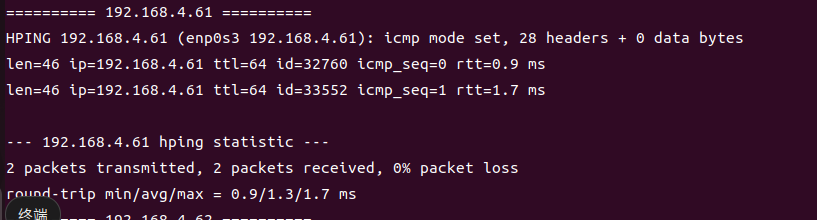
\includegraphics[width=0.86\linewidth]{figures/task12/第一台资产.png}
    \caption{ICMP 探测发现隐藏资产 \texttt{192.168.4.61}}
    \label{fig:task1-icmp-61}
\end{figure}

\begin{figure}[H]
    \centering
    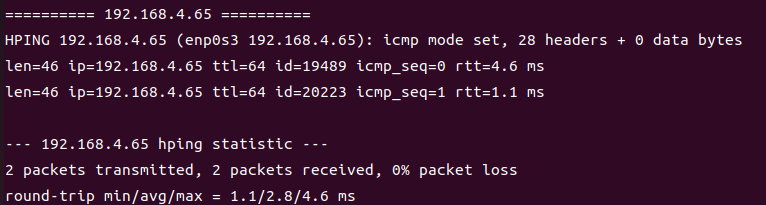
\includegraphics[width=0.86\linewidth]{figures/task12/第二台资产.png}
    \caption{ICMP 探测发现隐藏资产 \texttt{192.168.4.65}}
    \label{fig:task1-icmp-65}
\end{figure}

\begin{figure}[H]
    \centering
    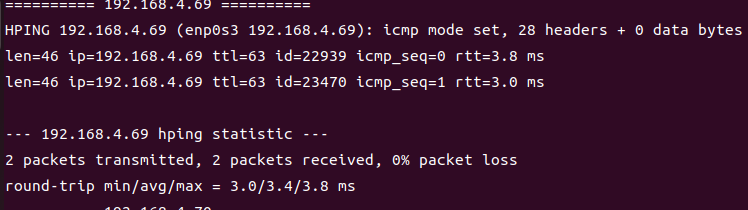
\includegraphics[width=0.86\linewidth]{figures/task12/第三台资产.png}
    \caption{ICMP 探测发现隐藏资产 \texttt{192.168.4.69}}
    \label{fig:task1-icmp-69}
\end{figure}

其余地址在本轮测试中均未收到回复。由此可以确定三台已响应的存活资产，但未收到 ICMP 回复并不必然意味着目标离线，也可能是探测报文被过滤。

\subsection{使用 \texttt{hping3} 进行 TCP 标志位探测}

按照实验指导，先针对 \texttt{192.168.4.61} 的 TCP 80 端口分别发送携带 SYN、ACK、PUSH、FIN、RST 标志位的报文，检查目标的 TCP 响应：

\begin{lstlisting}[language=bash,caption={对单个目标进行五种 TCP 标志位探测}]
sudo hping3 -S -I enp0s3 -p 80 -c 2 192.168.4.61
sudo hping3 -A -I enp0s3 -p 80 -c 2 192.168.4.61
sudo hping3 -P -I enp0s3 -p 80 -c 2 192.168.4.61
sudo hping3 -F -I enp0s3 -p 80 -c 2 192.168.4.61
sudo hping3 -R -I enp0s3 -p 80 -c 2 192.168.4.61
\end{lstlisting}

根据实际终端输出，各类型报文的响应如表~\ref{tab:task1-tcp-flags} 所示。

\begin{table}[H]
    \centering
    \caption{\texttt{192.168.4.61:80} 的 TCP 标志位探测结果}
    \label{tab:task1-tcp-flags}
    \renewcommand{\arraystretch}{1.2}
    \begin{tabularx}{\linewidth}{l c c X}
        \toprule
        发送标志位 & 返回标志位 & 收发结果 & 结果分析 \\
        \midrule
        SYN & RA & 2/2 & 收到 RST+ACK，表明主机有响应，80 端口关闭 \\
        ACK & R & 2/2 & 收到 RST，可说明有 TCP 响应，但无法单独判断端口开闭 \\
        PUSH & RA & 2/2 & 收到 RST+ACK，目标拒绝该报文 \\
        FIN & RA & 2/2 & 收到 RST+ACK，目标拒绝该报文 \\
        RST & 无 & 0/2 & 未收到应答；RST 报文通常不会再触发 TCP 回复 \\
        \bottomrule
    \end{tabularx}
\end{table}

其中，\texttt{flags=RA} 表示响应同时携带 RST 和 ACK 标志，说明目标的 TCP 协议栈确实收到了探测报文，但目标 TCP 80 端口没有建立相应连接。因此，端口关闭和主机离线是不同的概念，不能仅凭 80 端口未开放就认为主机不存在。

随后按照实验要求，对 \texttt{192.168.4.60--192.168.4.70} 整个区间发送 SYN 报文：

\begin{lstlisting}[language=bash,caption={使用 TCP SYN 批量探测资产区}]
for i in {60..70}; do
    echo "========== 192.168.4.$i =========="
    sudo hping3 -S -I enp0s3 -p 80 -c 2 192.168.4.$i
done
\end{lstlisting}

结果显示，\texttt{192.168.4.61}、\texttt{192.168.4.65} 和 \texttt{192.168.4.69} 均返回 \texttt{flags=RA}，每个目标均收到两次响应；区间内其余地址未收到回复。TCP SYN 探测与之前的 ICMP 发现结果一致，确认了三台隐藏主机。

\subsection{使用 \texttt{hping3} 进行 UDP 主机探测}

实验指导还要求通过 UDP 报文进行探测。UDP 是无连接协议，不存在 TCP 的 SYN/SYN-ACK 握手；若目标 UDP 端口没有服务监听，目标主机可能返回 ICMP Port Unreachable 差错报文，因此该响应也可以用来识别存活主机。

指导给出的 UDP 端口号为 \texttt{123456}，但源端口和目的端口字段均为 16 bit，合法端口号范围为 0 至 65535。因此本实验将目的端口改为 \texttt{12345}，实验指导中原参数的截图如图~\ref{fig:task1-udp-correction} 所示。

\begin{figure}[H]
    \centering
    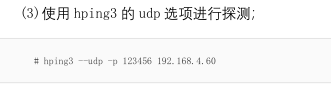
\includegraphics[width=0.73\linewidth]{figures/task12/纠正.png}
    \caption{实验指导中 UDP 目标端口参数的原始写法}
    \label{fig:task1-udp-correction}
\end{figure}

首先探测 \texttt{192.168.4.61}：

\begin{lstlisting}[language=bash,caption={针对单台主机的 UDP 探测}]
sudo hping3 --udp -I enp0s3 -p 12345 -c 2 192.168.4.61
\end{lstlisting}

该主机返回两条 \texttt{ICMP Port Unreachable}，如图~\ref{fig:task1-udp} 所示。该结果表明目标主机可达，但被探测的 UDP 端口未提供可接受该数据报的服务。

\begin{figure}[H]
    \centering
    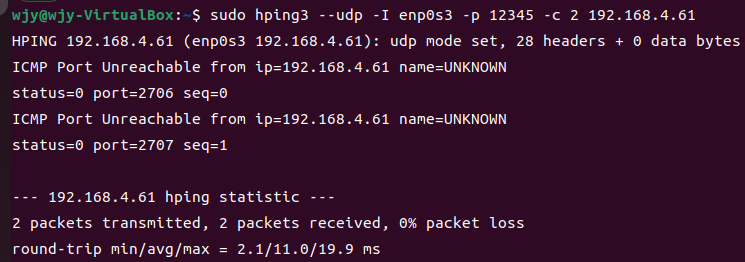
\includegraphics[width=0.84\linewidth]{figures/task12/UDP测试结果.png}
    \caption{对 \texttt{192.168.4.61} 进行 UDP 探测并收到端口不可达响应}
    \label{fig:task1-udp}
\end{figure}

继续遍历完整目标区间：

\begin{lstlisting}[language=bash,caption={UDP 批量主机探测}]
for i in {60..70}; do
    echo "========== 192.168.4.$i =========="
    sudo hping3 --udp -I enp0s3 -p 12345 -c 2 192.168.4.$i
done
\end{lstlisting}

根据实际输出，\texttt{192.168.4.61}、\texttt{192.168.4.65} 和 \texttt{192.168.4.69} 均返回 ICMP Port Unreachable，且各收到两次响应；其他被测地址没有响应。至此，ICMP、TCP SYN 与 UDP 三种方式均探测出相同的三台隐藏主机。需要注意，对于 UDP 探测，无响应同样不能直接等同于主机离线。

\subsection{使用 \texttt{Nmap} 进行主机发现及服务识别}

\subsubsection{资产区主机存活探测}

按照实验指导，使用 \texttt{Nmap} 的 \texttt{-sn} 参数扫描完整资产区 \texttt{192.168.4.0/24}，仅进行主机发现而不执行常规端口扫描：

\begin{lstlisting}[language=bash,caption={Nmap 对整个资产区进行主机发现}]
sudo nmap -sn 192.168.4.0/24
\end{lstlisting}

最终扫描显示共检查 256 个 IP 地址，其中 5 台主机存活，分别为 \texttt{192.168.4.1}、\texttt{192.168.4.61}、\texttt{192.168.4.65}、\texttt{192.168.4.69} 和 \texttt{192.168.4.105}，实际结果如图~\ref{fig:task1-nmap-alive} 所示。

\begin{figure}[H]
    \centering
    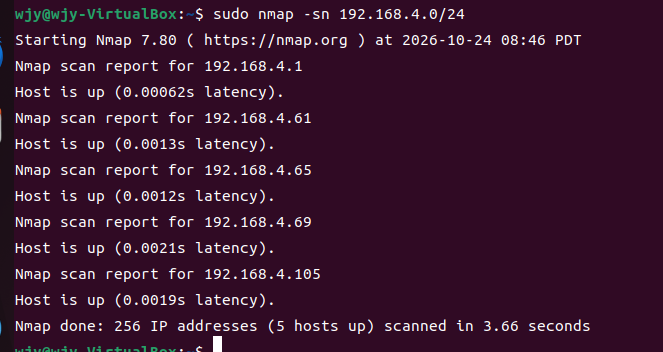
\includegraphics[width=0.84\linewidth]{figures/task12/Nmap结果.png}
    \caption{Nmap 发现资产区中的 5 台存活设备}
    \label{fig:task1-nmap-alive}
\end{figure}

与 \texttt{hping3} 相比，Nmap 一次可以扫描整个网段，并结合多种探测方式判断存活状态。因此，扫描结果不仅包括三台隐藏资产，还包括资产区网关和 Web 服务器。

\subsubsection{操作系统与服务版本识别}

接着按照实验指导使用 TCP SYN 扫描、操作系统识别和服务版本检测：

\begin{lstlisting}[language=bash,caption={Nmap 资产详细信息扫描}]
sudo nmap -sS 192.168.4.0/24 -O -A -sV
\end{lstlisting}

其中，\texttt{-sS} 表示 TCP SYN 扫描，\texttt{-O} 表示操作系统识别，\texttt{-sV} 表示服务版本探测；\texttt{-A} 还会开启版本识别、操作系统检测、默认脚本及路由跟踪等功能。保留这些参数是为了与实验指导中的命令一致。

实际扫描显示：OpenWRT 的 \texttt{22/tcp} 开放 Dropbear SSH 服务，\texttt{53/tcp} 开放 DNS 服务；三台隐藏资产在默认扫描的 1000 个 TCP 端口上均显示为关闭；Web 服务器 \texttt{192.168.4.105} 的 \texttt{80/tcp} 开放 Apache httpd 2.4.52 服务。

需要注意，Nmap 对多个目标报告 \texttt{No exact OS matches} 或 \texttt{Too many fingerprints match this host}，未能精确识别操作系统。因此下文的操作系统名称应结合虚拟机实际部署情况填写，不能将其表述为 Nmap 独立识别的结果。

\subsection{服务器全 TCP 端口扫描}

最后按照实验指导，对目标服务器 \texttt{192.168.4.105} 进行全端口扫描：

\begin{lstlisting}[language=bash,caption={服务器 65535 个 TCP 端口扫描}]
sudo nmap 192.168.4.105 -p- -O -A -sV
\end{lstlisting}

其中 \texttt{-p-} 指定扫描全部 65535 个 TCP 端口，而不是 Nmap 默认选择的常见端口。此次扫描的关键输出如下：

\begin{lstlisting}[caption={服务器全端口扫描的实际关键输出}]
Nmap scan report for 192.168.4.105
Host is up (0.0014s latency).
Not shown: 65534 closed ports
PORT   STATE SERVICE VERSION
80/tcp open  http    Apache httpd 2.4.52
|_http-server-header: Apache/2.4.52 (Ubuntu)
|_http-title: 401 Unauthorized
\end{lstlisting}

由此可知，服务器的 65535 个 TCP 端口中仅 \texttt{80/tcp} 开放，其余 65534 个端口均处于关闭状态。HTTP 检测返回 \texttt{401 Unauthorized}，说明 Apache 服务能够接收并回应请求，但当前访问需要身份认证，并不表示 Web 服务未启动。

\subsection{资产及端口信息统计}

\subsubsection{资产信息统计}

根据主机发现和详细扫描结果，并结合实验环境中实际部署的系统类型，填写实验指导中的资产信息统计表，如表~\ref{tab:task1-assets} 所示。

\begin{table}[H]
    \centering
    \caption{资产信息统计}
    \label{tab:task1-assets}
    \renewcommand{\arraystretch}{1.2}
    \begin{tabularx}{\linewidth}{l l X}
        \toprule
        存活主机 IP & 设备类型 & 操作系统 \\
        \midrule
        \texttt{192.168.4.1} & 路由器 & OpenWRT（Linux） \\
        \texttt{192.168.4.61} & 普通主机（Victim） & Ubuntu Linux \\
        \texttt{192.168.4.65} & 普通主机（User） & Ubuntu Linux \\
        \texttt{192.168.4.69} & 普通主机（HostC） & Ubuntu Linux \\
        \texttt{192.168.4.105} & Web 服务器 & Ubuntu Linux \\
        \bottomrule
    \end{tabularx}
\end{table}

其中操作系统信息来自已知虚拟机部署情况；Nmap 本次只完成了存活主机及部分服务的识别，没有对所有主机给出精确的操作系统指纹结论。

\subsubsection{服务器端口信息统计}

服务器全端口扫描结果对应实验指导中的端口信息统计表，见表~\ref{tab:task1-ports}。

\begin{table}[H]
    \centering
    \caption{服务器 \texttt{192.168.4.105} 的端口信息统计}
    \label{tab:task1-ports}
    \renewcommand{\arraystretch}{1.2}
    \begin{tabularx}{\linewidth}{l l X}
        \toprule
        统计项目 & \texttt{80/tcp} & 其余 65534 个 TCP 端口 \\
        \midrule
        开放状态 & open（开放） & closed（关闭） \\
        服务及版本 & Apache httpd 2.4.52 & 无开放服务 \\
        \bottomrule
    \end{tabularx}
\end{table}

本实验通过 \texttt{hping3} 的 ICMP、TCP、UDP 三类探测发现了三台隐藏资产，再利用 Nmap 识别资产区的五台存活设备，并确认 Web 服务器只开放 \texttt{80/tcp} 端口。三种协议得到的主机发现结果一致，但依赖的响应机制不同；在分析探测结果时，应将主机存活、端口状态和服务版本分别判断。


% \section{实验三：\texttt{TCP} 连接重置}

\subsection{实验环境与网络配置}

本实验在 WSL2 中使用 Docker Compose 搭建隔离网络。拓扑包含攻击者、用户、路由器、受害者服务器和正常服务器。攻击者、用户分别位于不同网段；两台服务器位于同一服务器网段，由路由器转发用户与服务器之间的流量。各节点地址如表~\ref{tab:task3-network} 所示。

\begin{table}[H]
    \centering
    \caption{\texttt{TCP} 连接重置实验的实际网络配置}
    \label{tab:task3-network}
    \renewcommand{\arraystretch}{1.2}
    \begin{tabularx}{\linewidth}{l l l X}
        \toprule
        节点 & 网段侧 & IPv4 地址 & 默认路由 \\
        \midrule
        Attacker & 攻击者网段 & \texttt{192.168.2.100/24} & \texttt{192.168.2.10} \\
        User & 用户网段 & \texttt{192.168.3.100/24} & \texttt{192.168.3.10} \\
        Router & 攻击者侧 & \texttt{192.168.2.10/24} & -- \\
        Router & 用户侧 & \texttt{192.168.3.10/24} & -- \\
        Router & 服务器侧 & \texttt{192.168.4.10/24} & -- \\
        Victim Server & 服务器网段 & \texttt{192.168.4.105/24} & \texttt{192.168.4.10} \\
        Normal Server & 服务器网段 & \texttt{192.168.4.106/24} & \texttt{192.168.4.10} \\
        \bottomrule
    \end{tabularx}
\end{table}

路由器开启 IPv4 转发，并使用 Linux 流量控制（\texttt{tc}）把用户侧和服务器侧入口的 IPv4 报文镜像到攻击者侧。Docker 网络关闭源地址伪装，因而镜像报文仍保留 User 和服务器的原始 IP 地址。Attacker 上的 Scapy 脚本只处理从受害者服务器发往 User 的 \texttt{TCP} 报文，并从中读取端口和确认号。

\subsection{攻击前的连通性检查}

开始攻击前，User 分别访问受害者服务器和正常服务器。\texttt{HTTP} 请求均得到 \texttt{HTTP/1.1 200 OK}，\texttt{SSH}、\texttt{Telnet} 和 \texttt{FTP} 也均可建立连接并完成登录，作为后续对照。以下截图中的标记标出了相关客户端命令。\texttt{HTTP} 检查结果如图~\ref{fig:task3-http-before} 所示。

\begin{figure}[H]
    \centering
    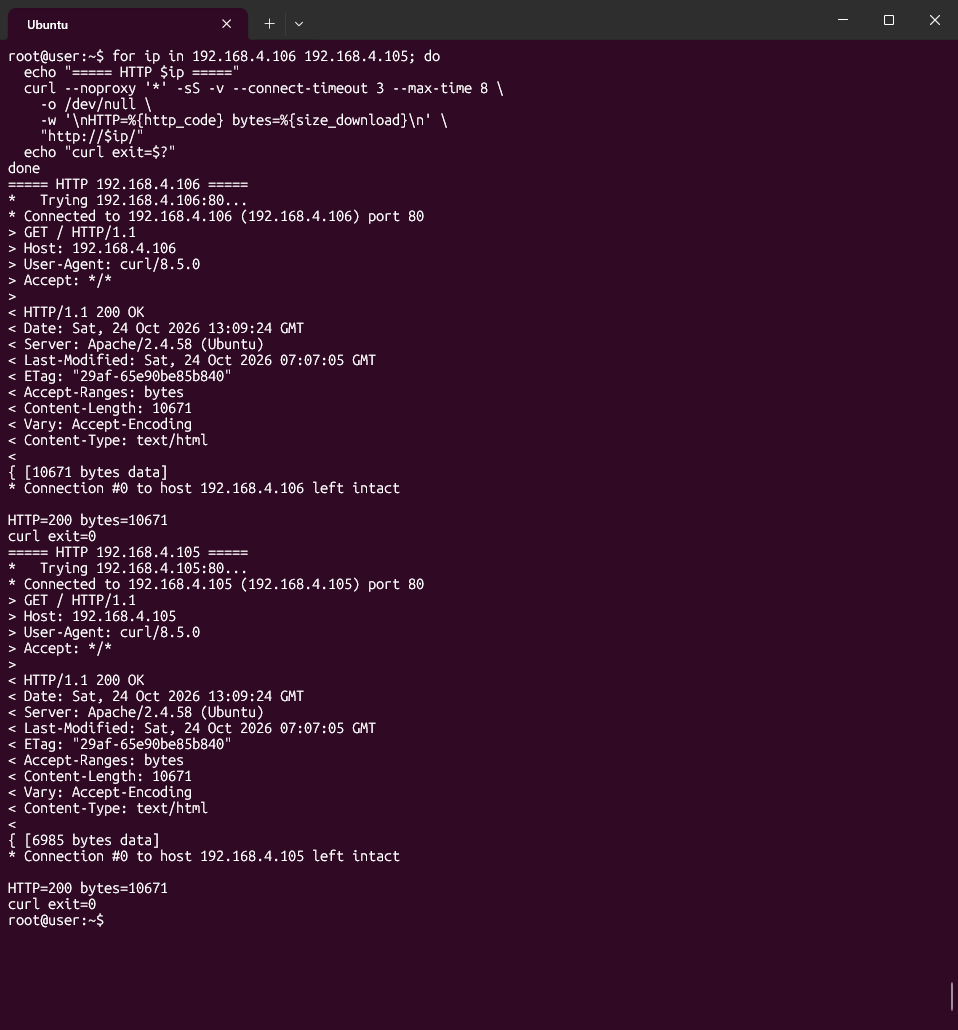
\includegraphics[width=0.86\linewidth]{figures/task3/http_before_attack.png}
    \caption{攻击前，User 能正常访问两台服务器的 \texttt{HTTP} 服务}
    \label{fig:task3-http-before}
\end{figure}

\texttt{Telnet} 登录结果如图~\ref{fig:task3-telnet-before} 所示，User 先后登录了正常服务器和受害者服务器，并能在两端执行命令。

\begin{figure}[H]
    \centering
    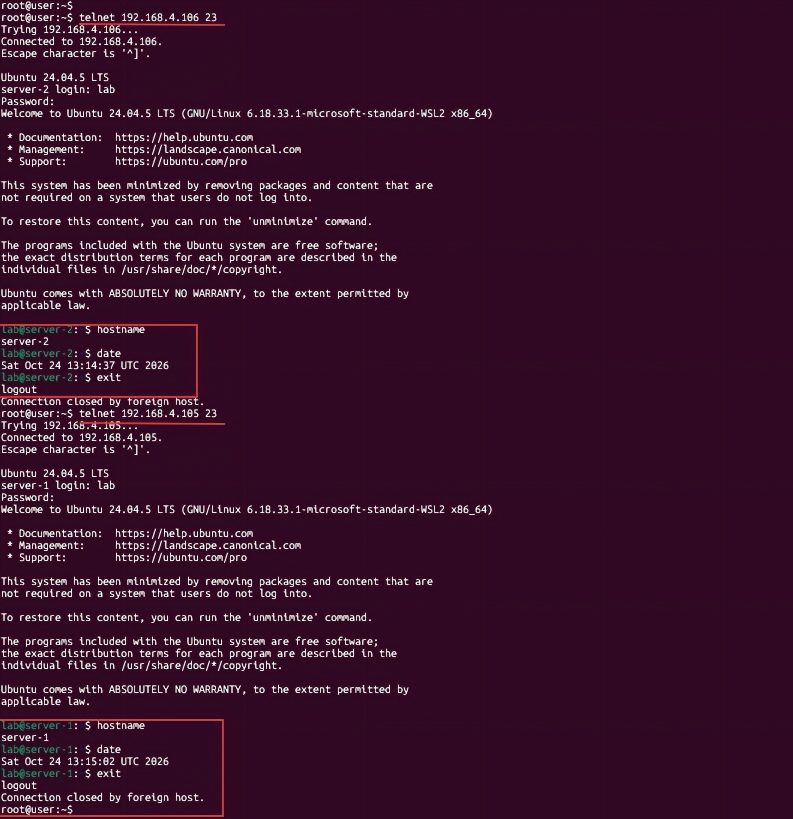
\includegraphics[width=0.78\linewidth]{figures/task3/telnet_before_attack(1).png}
    \caption{攻击前，User 分别成功登录两台服务器的 \texttt{Telnet} 服务}
    \label{fig:task3-telnet-before}
\end{figure}

\texttt{SSH} 检查中，User 分别连接到两台服务器并显示各自的主机名，说明攻击前两条 \texttt{SSH} 连接均可正常使用，如图~\ref{fig:task3-ssh-before} 所示。

\begin{figure}[H]
    \centering
    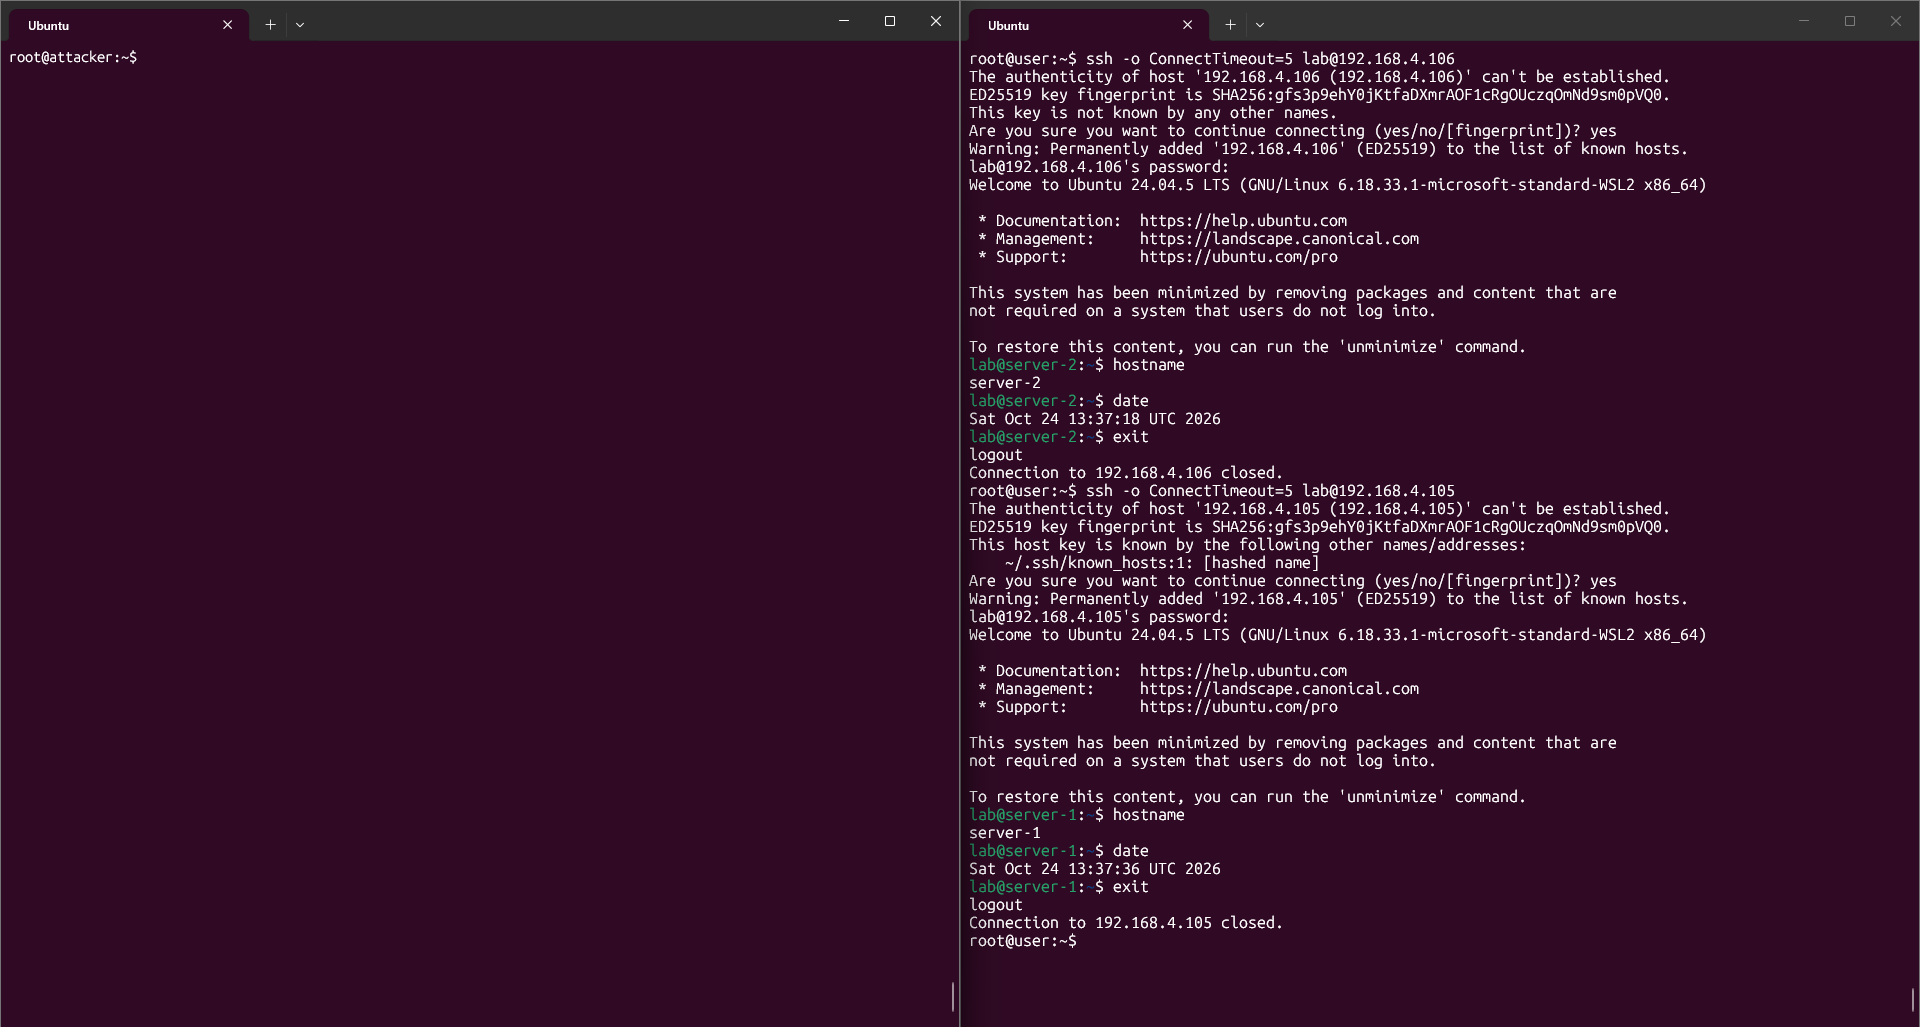
\includegraphics[trim=720bp 0 0 0,clip,width=0.88\linewidth]{figures/task3/ssh_before_attack.png}
    \caption{攻击前，User 分别通过 \texttt{SSH} 登录正常服务器和受害者服务器}
    \label{fig:task3-ssh-before}
\end{figure}

\texttt{FTP} 检查中，两台服务器均返回登录成功和目录列表，结果如图~\ref{fig:task3-ftp-before} 所示。

\begin{figure}[H]
    \centering
    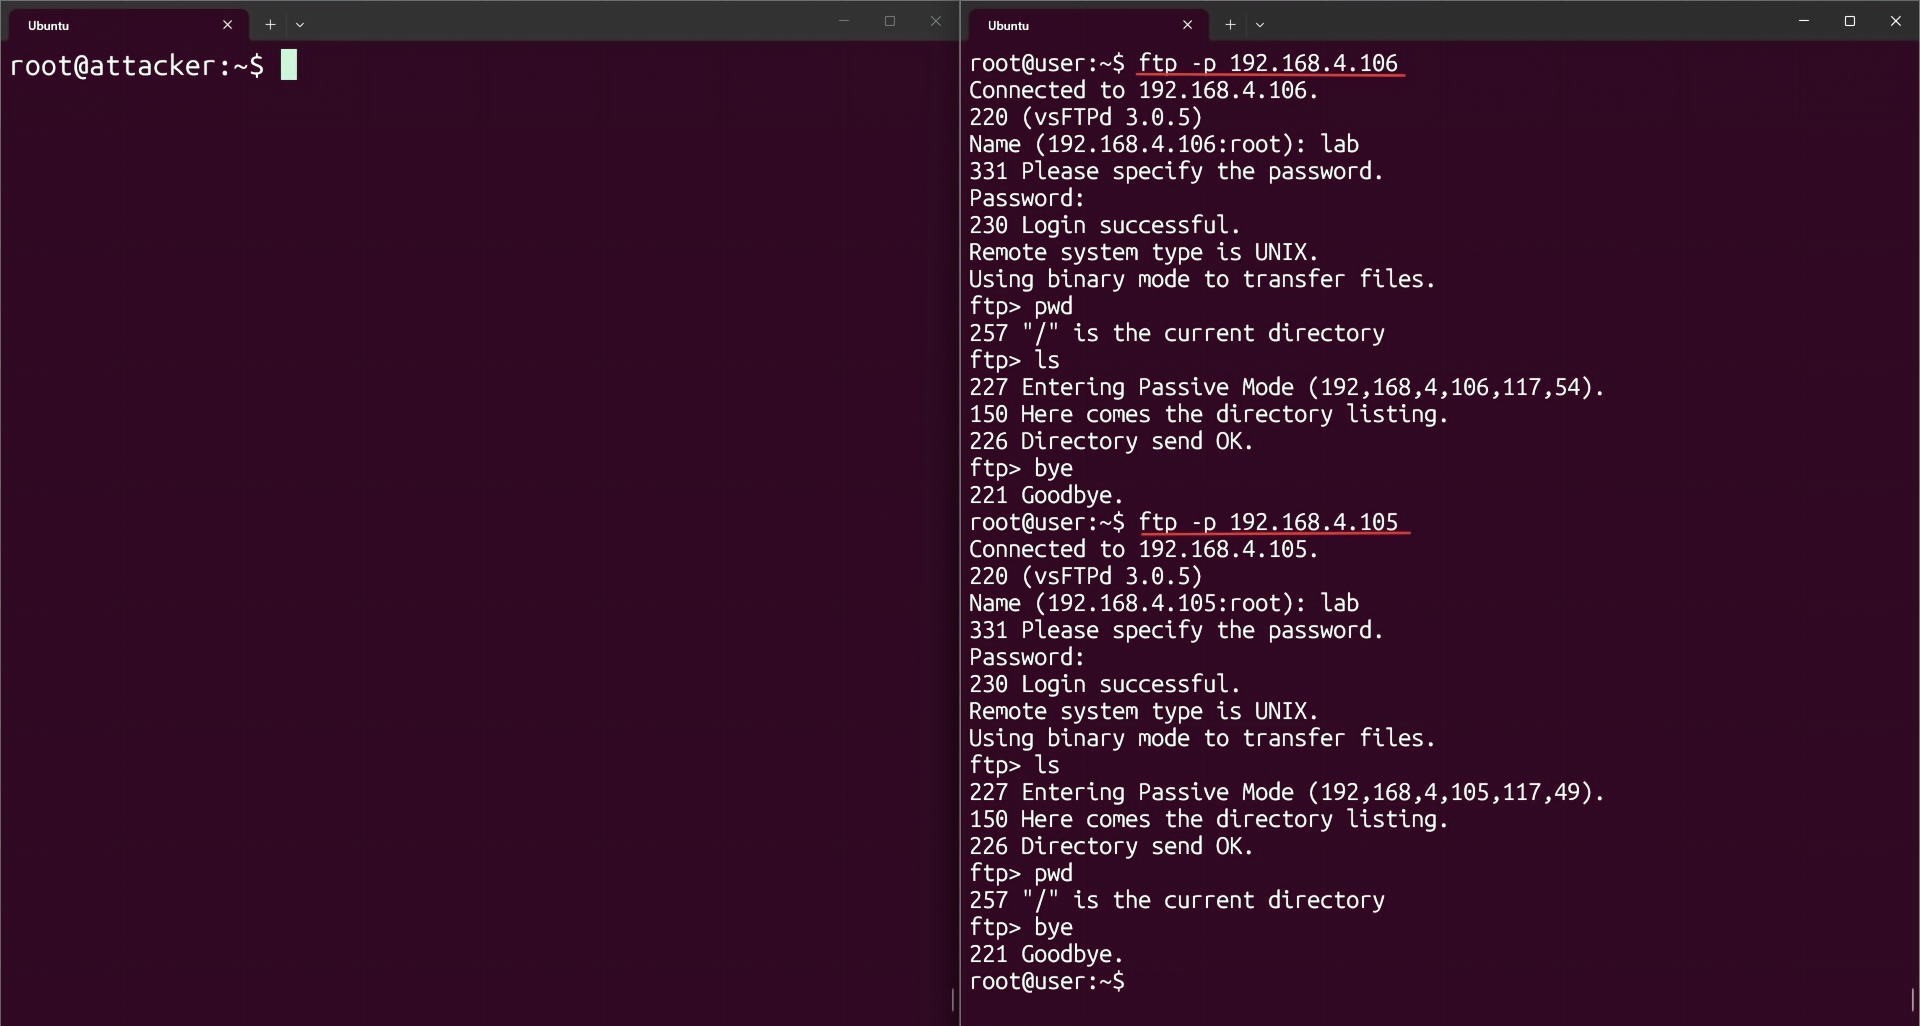
\includegraphics[trim=720bp 0 0 0,clip,width=0.88\linewidth]{figures/task3/ftp_before_attack(1).png}
    \caption{攻击前，User 均可登录两台服务器的 \texttt{FTP} 服务}
    \label{fig:task3-ftp-before}
\end{figure}

\subsection{监听流量并构造 \texttt{TCP} RST 报文}

在 Attacker 上运行 Scapy 监听脚本后，脚本使用如下过滤条件捕获从受害者服务器发往 User 的 \texttt{TCP} 报文：

\begin{lstlisting}[language=Python,caption={捕获服务器发往 User 的 \texttt{TCP} 流量}]
capture_filter = (
    "tcp and src host 192.168.4.105 "
    "and dst host 192.168.3.100"
)
\end{lstlisting}

回调函数从捕获报文中读取 \texttt{TCP} 源、目的端口和确认号，将 IP 地址及端口方向反转，并把服务器报文中的确认号作为伪造 RST 的序列号。脚本只对带 ACK 标志的报文发送 RST，核心处理如下：

\begin{lstlisting}[language=Python,caption={根据捕获到的确认号构造 \texttt{TCP} RST 报文}]
def packet_callback(packet):
    if not (packet.haslayer(IP) and packet.haslayer(TCP)):
        return

    tcp_layer = packet[TCP]
    if not (int(tcp_layer.flags) & 0x10):
        return

    reset_packet = (
        IP(src=USER_IP, dst=VICTIM_IP)
        / TCP(
            sport=int(tcp_layer.dport),
            dport=int(tcp_layer.sport),
            flags="R",
            seq=int(tcp_layer.ack),
        )
    )
    send(reset_packet, iface=ATTACKER_INTERFACE, verbose=False)

sniff(
    iface=ATTACKER_INTERFACE,
    filter=CAPTURE_FILTER,
    prn=packet_callback,
    store=False,
)
\end{lstlisting}

脚本启动后，User 分别使用 \texttt{HTTP}、\texttt{SSH}、\texttt{Telnet} 和 \texttt{FTP} 访问正常服务器及受害者服务器。攻击者终端显示其持续捕获服务器响应并发送以 User 为源地址、受害者服务器为目的地址的 RST 报文。

\subsection{不同 \texttt{TCP} 服务的攻击结果}

\subsubsection{\texttt{Telnet}、\texttt{SSH} 与 \texttt{FTP}}

\texttt{Telnet} 对照结果显示，攻击期间 User 仍能登录正常服务器 \texttt{192.168.4.106}；连接受害者服务器 \texttt{192.168.4.105} 时，服务器登录过程被中断，连接随即关闭，如图~\ref{fig:task3-telnet-after} 所示。

\begin{figure}[H]
    \centering
    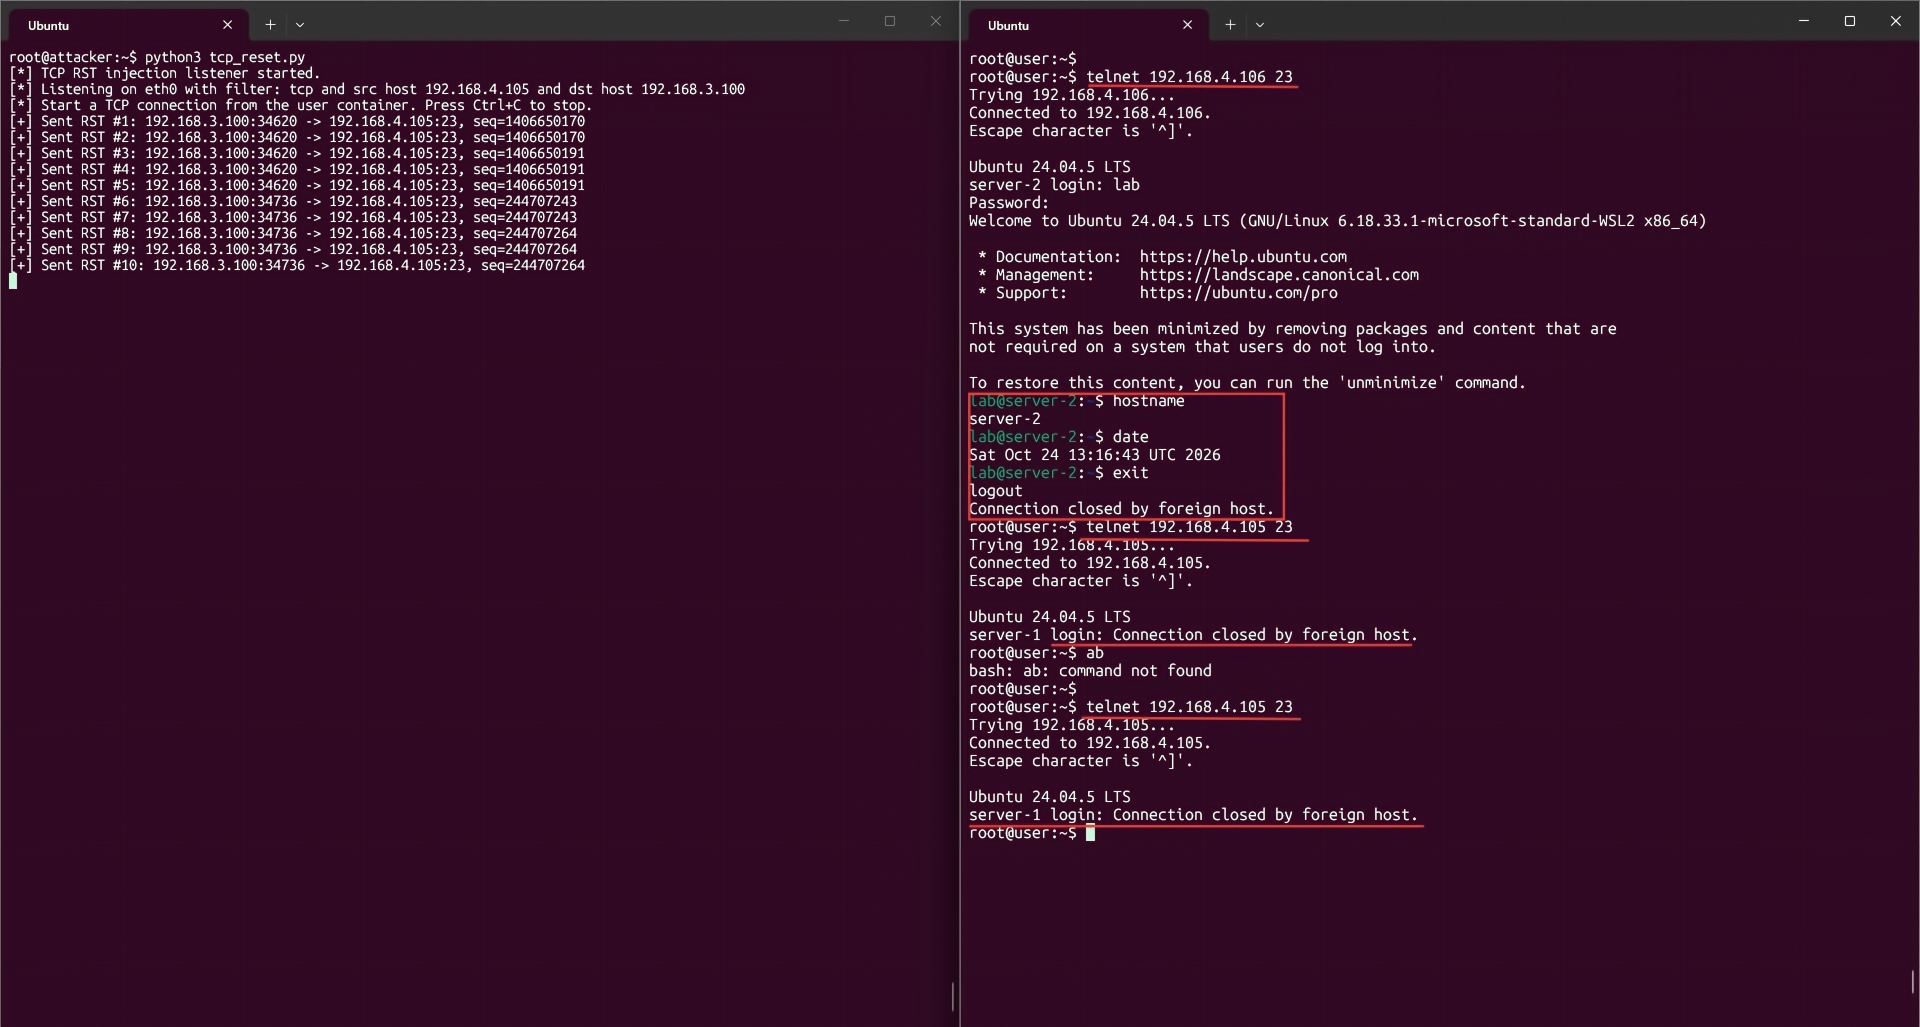
\includegraphics[trim=720bp 0 0 0,clip,width=0.88\linewidth]{figures/task3/telnet_after_attack(1).png}
    \caption{\texttt{TCP} 重置期间，正常服务器 \texttt{Telnet} 可用，受害者服务器连接被重置}
    \label{fig:task3-telnet-after}
\end{figure}

\texttt{SSH} 的结果与 \texttt{Telnet} 一致：正常服务器仍可登录，而连接受害者服务器时出现 \texttt{Connection reset by 192.168.4.105}，如图~\ref{fig:task3-ssh-after} 所示。

\begin{figure}[H]
    \centering
    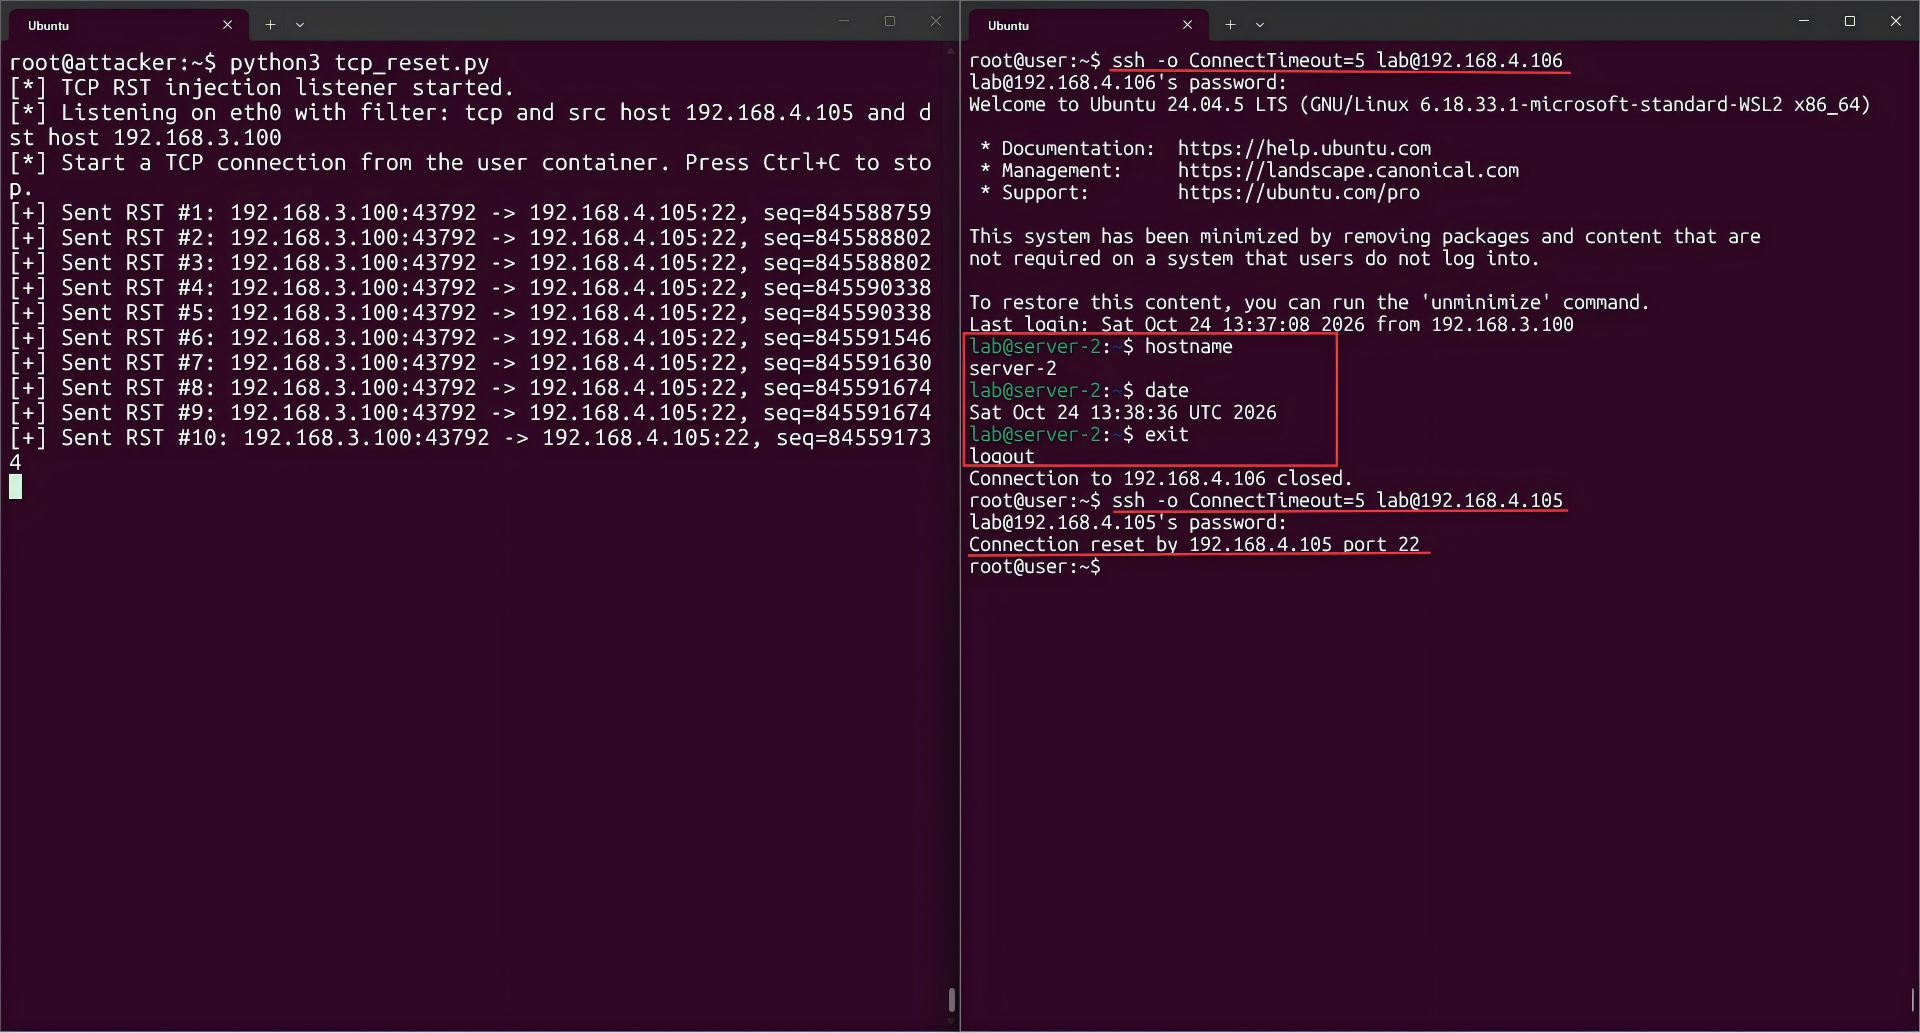
\includegraphics[trim=720bp 0 0 0,clip,width=0.88\linewidth]{figures/task3/ssh_after_attack(1).png}
    \caption{\texttt{TCP} 重置期间，正常服务器 \texttt{SSH} 可用，受害者服务器连接被重置}
    \label{fig:task3-ssh-after}
\end{figure}

\texttt{FTP} 对照中，正常服务器仍能完成登录和目录查询；受害者服务器的控制连接则返回 \texttt{421 Service not available} 并关闭。Attacker 终端同时记录到发往受害者 \texttt{FTP} 端口 21 的 RST 报文，如图~\ref{fig:task3-ftp-after} 所示。

\begin{figure}[H]
    \centering
    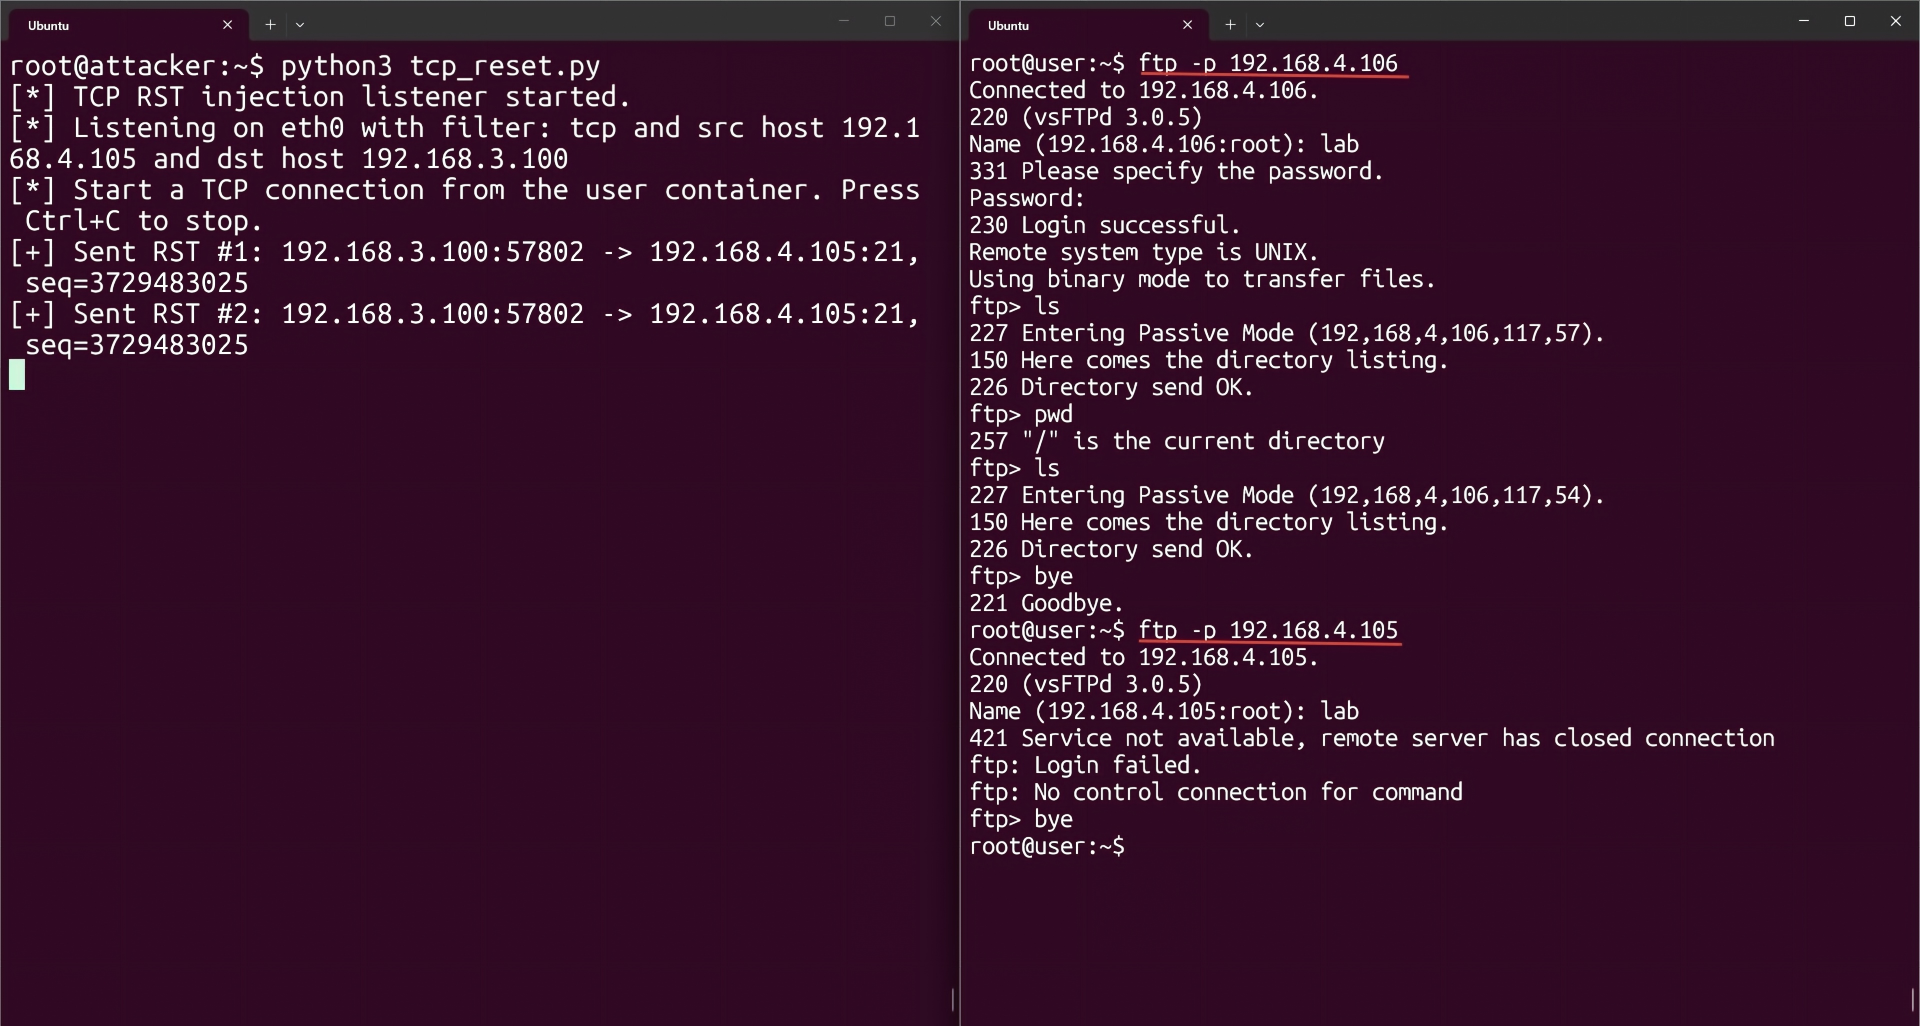
\includegraphics[width=0.98\linewidth]{figures/task3/ftp_after_attack(1).png}
    \caption{\texttt{TCP} 重置期间，正常服务器 \texttt{FTP} 可用，受害者服务器 \texttt{FTP} 连接关闭}
    \label{fig:task3-ftp-after}
\end{figure}

\subsubsection{\texttt{HTTP} 下载及响应时序}
在 \texttt{HTTP} 的攻击测试中，为了使攻击效果更显著，这里在两个 Server 上都上传了大小为 8MB 的数据文件，使用 \texttt{HTTP} 从服务器下载文件，大约需要 32s 左右的时间，足够充分体现攻击效果。
首次 \texttt{HTTP} 测试中，受害者服务器返回的页面大小为 10\,671 字节。虽然 Attacker 已经发送 RST，User 仍收到了完整页面，curl 返回状态为 0，如图~\ref{fig:task3-http-small} 所示。这表明对于传输很快结束的小响应，RST 可能在下载完成后才到达，因而未能中断该次请求。

\begin{figure}[H]
    \centering
    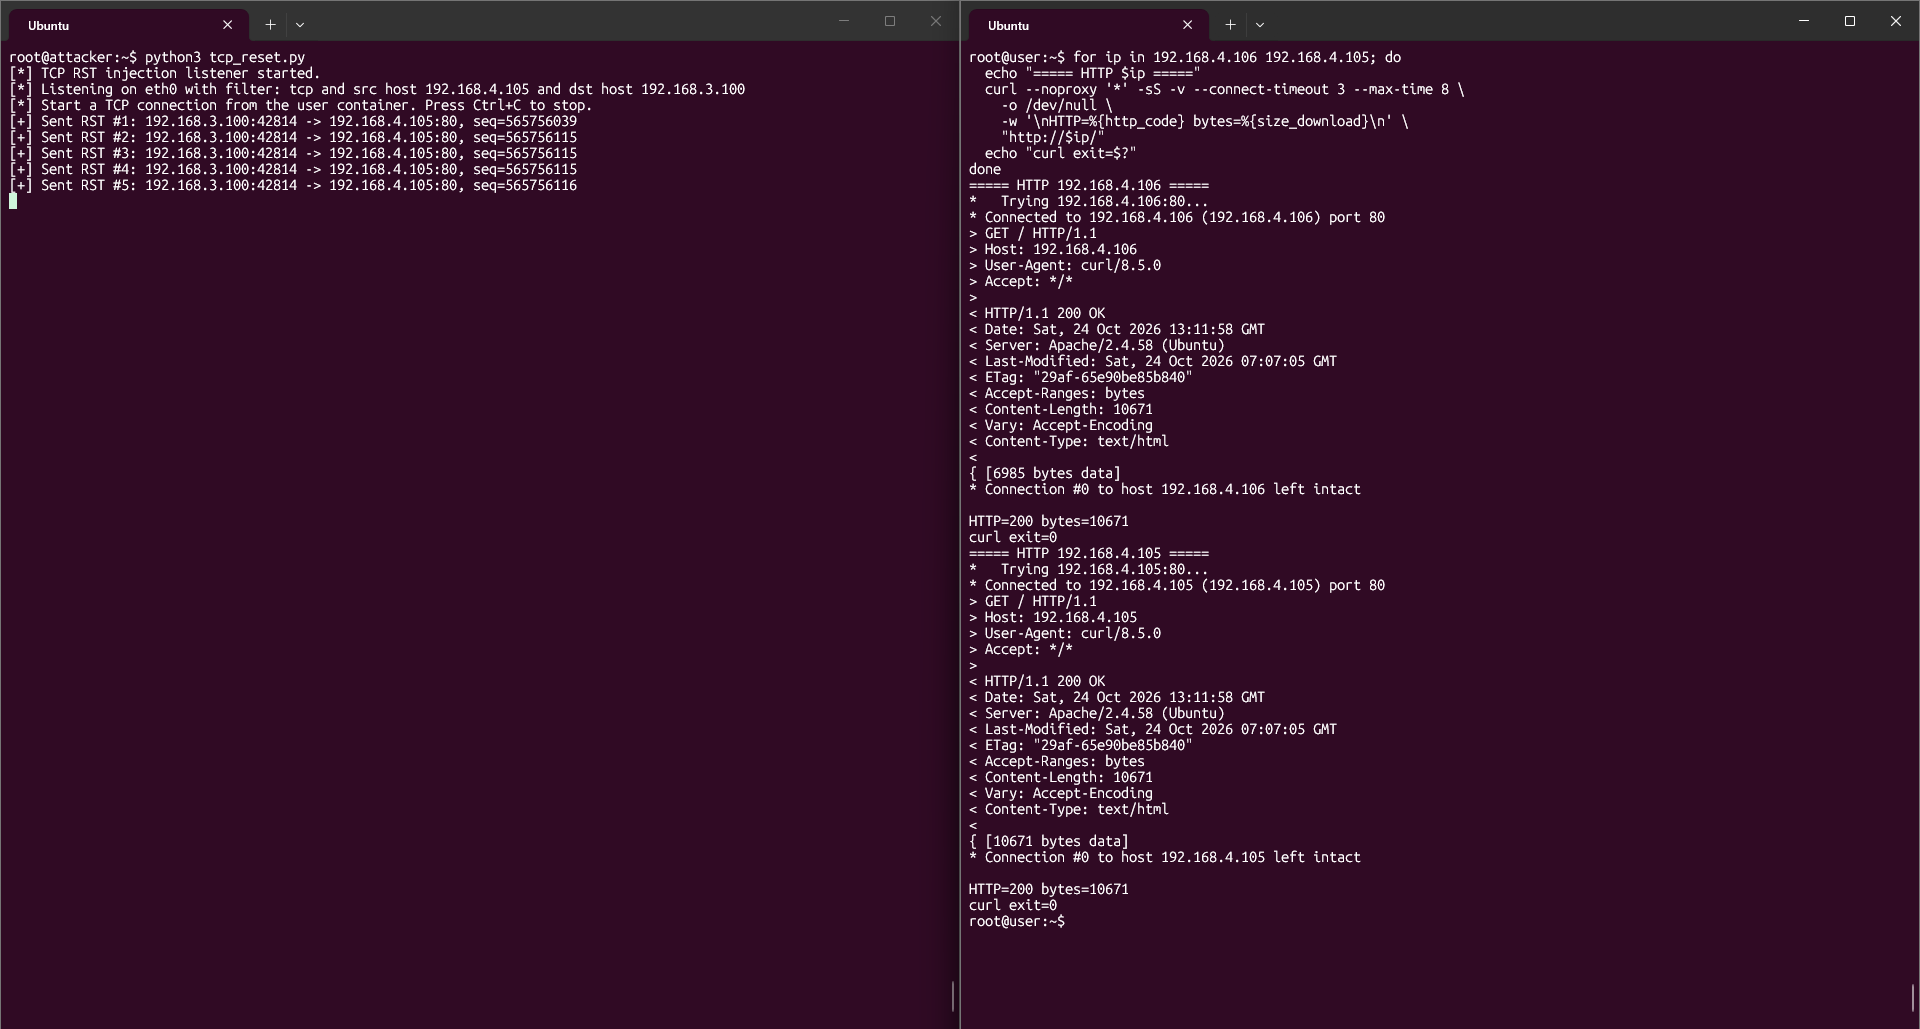
\includegraphics[width=0.98\linewidth]{figures/task3/http_short_response.png}
    \caption{小型 \texttt{HTTP} 响应在 RST 生效前完成传输}
    \label{fig:task3-http-small}
\end{figure}

为观察持续时间更长的连接，随后使用限速方式下载约 8\,MiB 的测试文件。攻击前，User 从两台服务器下载该文件均得到 \texttt{HTTP 200}，并完整收到 8\,388\,608 字节，如图~\ref{fig:task3-http-large-before} 所示。

\begin{figure}[H]
    \centering
    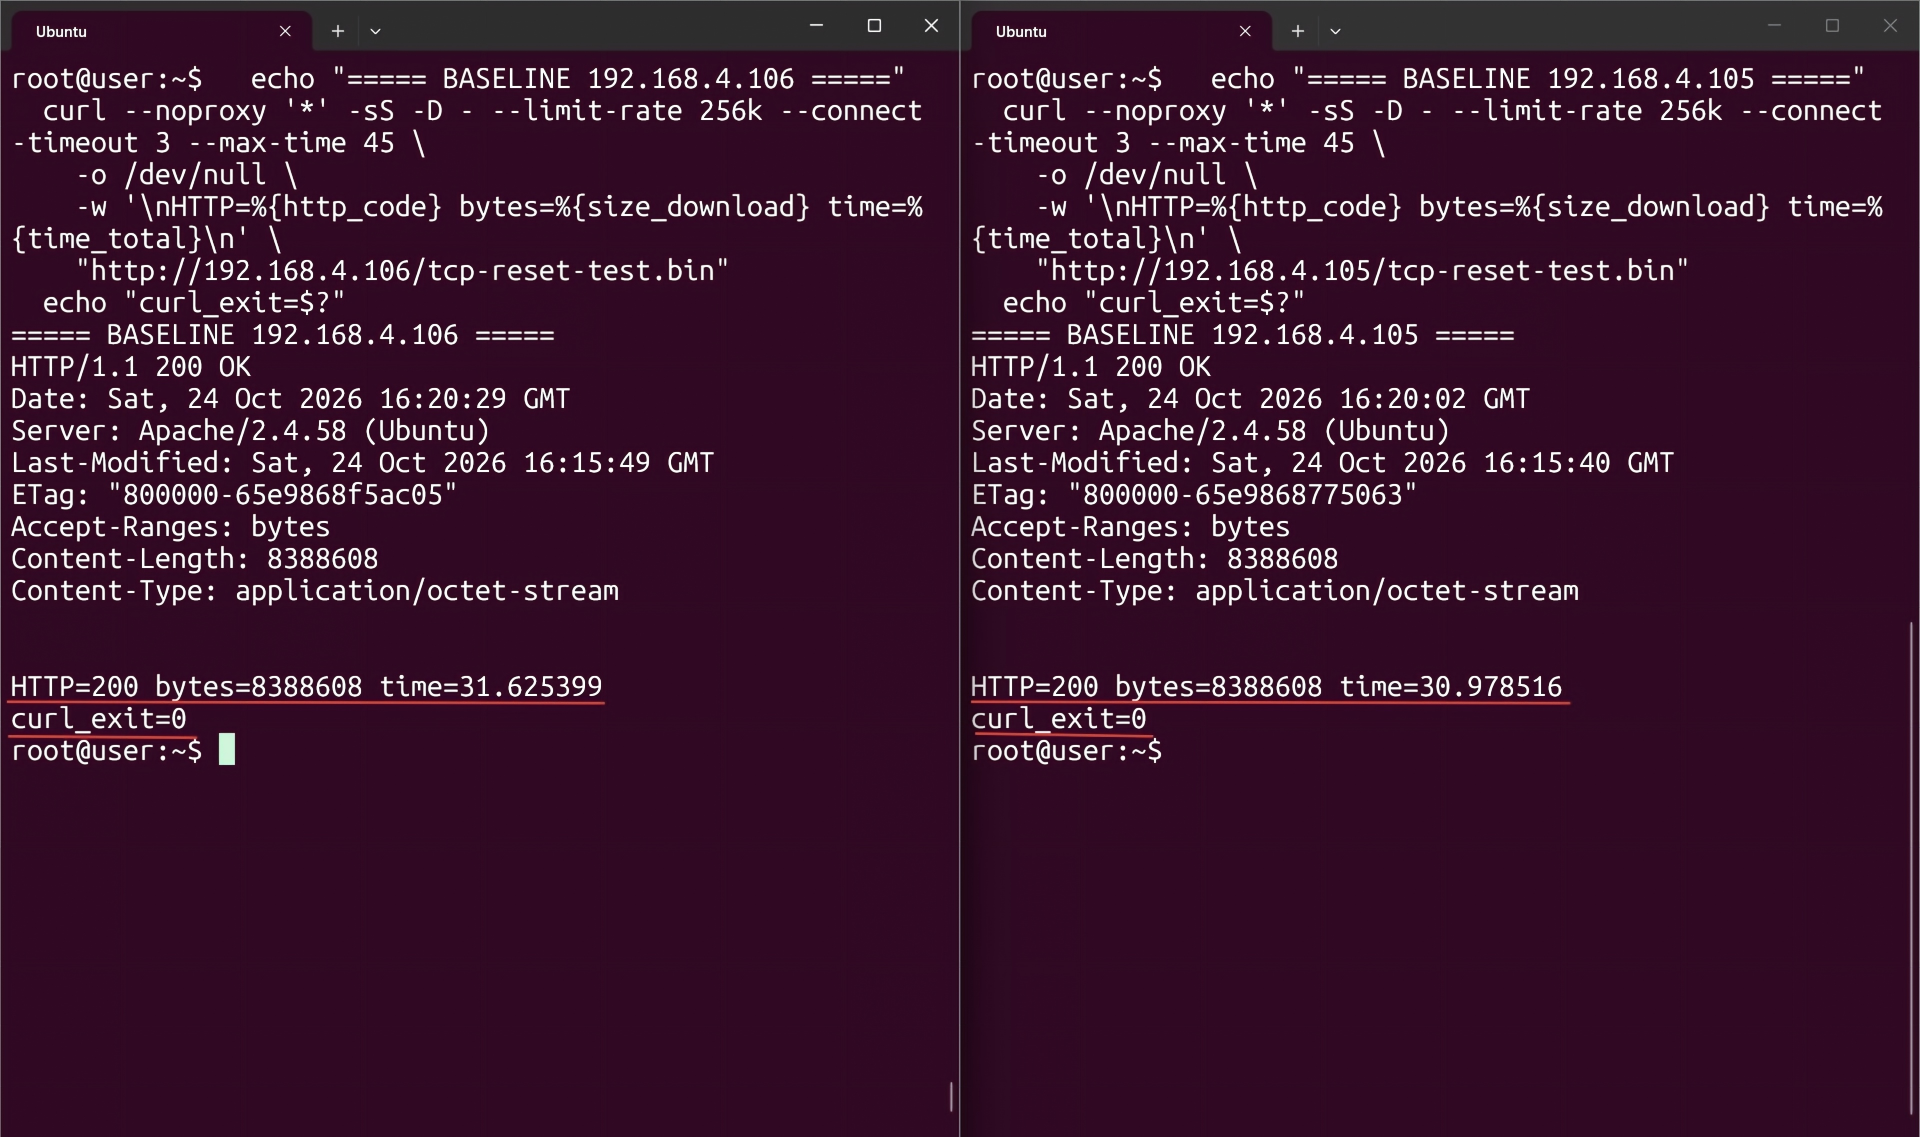
\includegraphics[width=0.98\linewidth]{figures/task3/http_large_before_attack(1).png}
    \caption{攻击前，User 均能完整下载两台服务器提供的测试文件}
    \label{fig:task3-http-large-before}
\end{figure}

启动 RST 监听后，正常服务器的下载仍完整结束，curl 返回状态为 0；从受害者服务器下载时，连接被重置，只收到 2\,725\,685 字节，curl 返回状态为 56。对照结果和 Attacker 的 RST 发送记录见图~\ref{fig:task3-http-after}。

\begin{figure}[H]
    \centering
    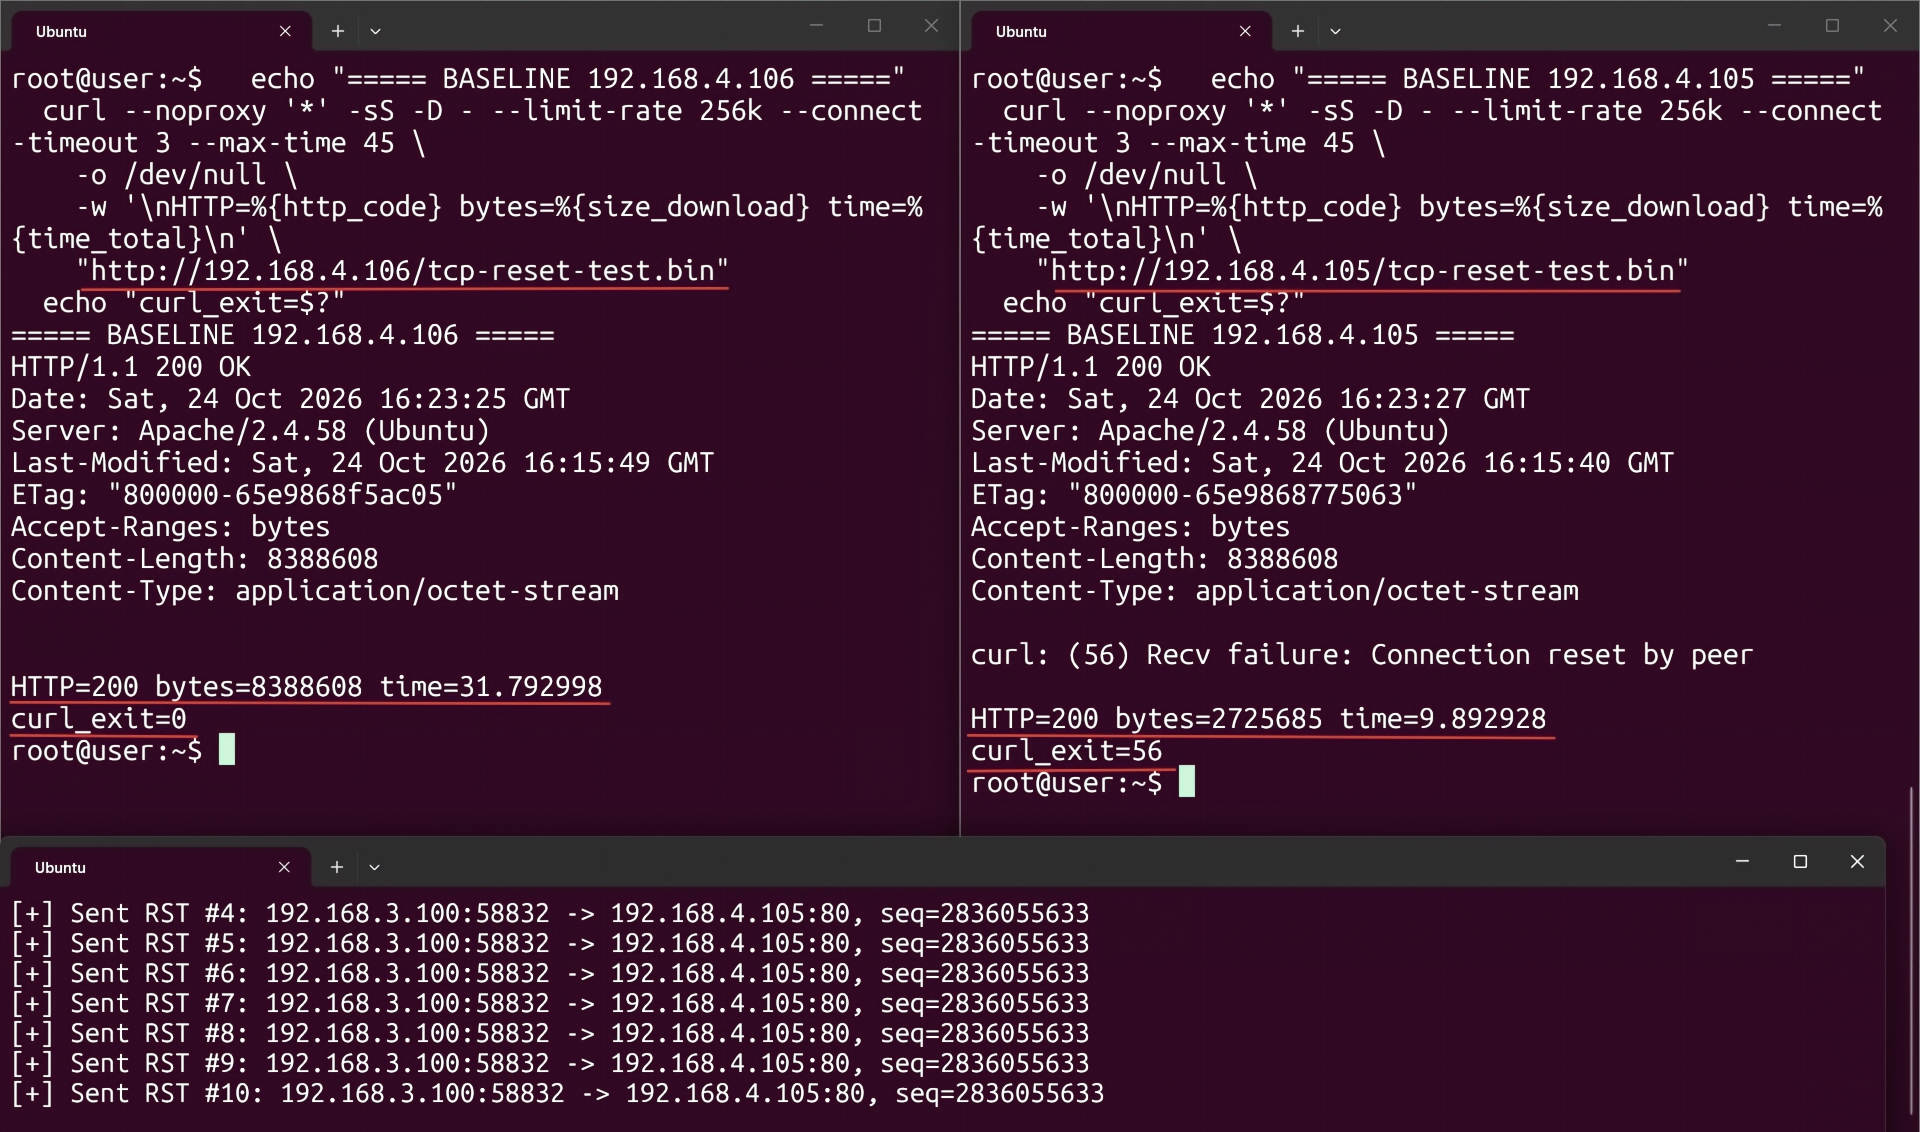
\includegraphics[width=0.98\linewidth]{figures/task3/http_reset_effect(1).png}
    \caption{限速 \texttt{HTTP} 下载时，受害者服务器连接中断，正常服务器下载完成}
    \label{fig:task3-http-after}
\end{figure}

\subsection{停止攻击后的恢复验证}

停止 Attacker 上的监听脚本后，再次从受害者服务器下载同一测试文件。User 收到完整的 8\,388\,608 字节，curl 返回状态为 0，说明停止发送伪造 RST 后，受害者服务器的 \texttt{HTTP} 连接恢复正常，如图~\ref{fig:task3-recovery} 所示。

\begin{figure}[H]
    \centering
    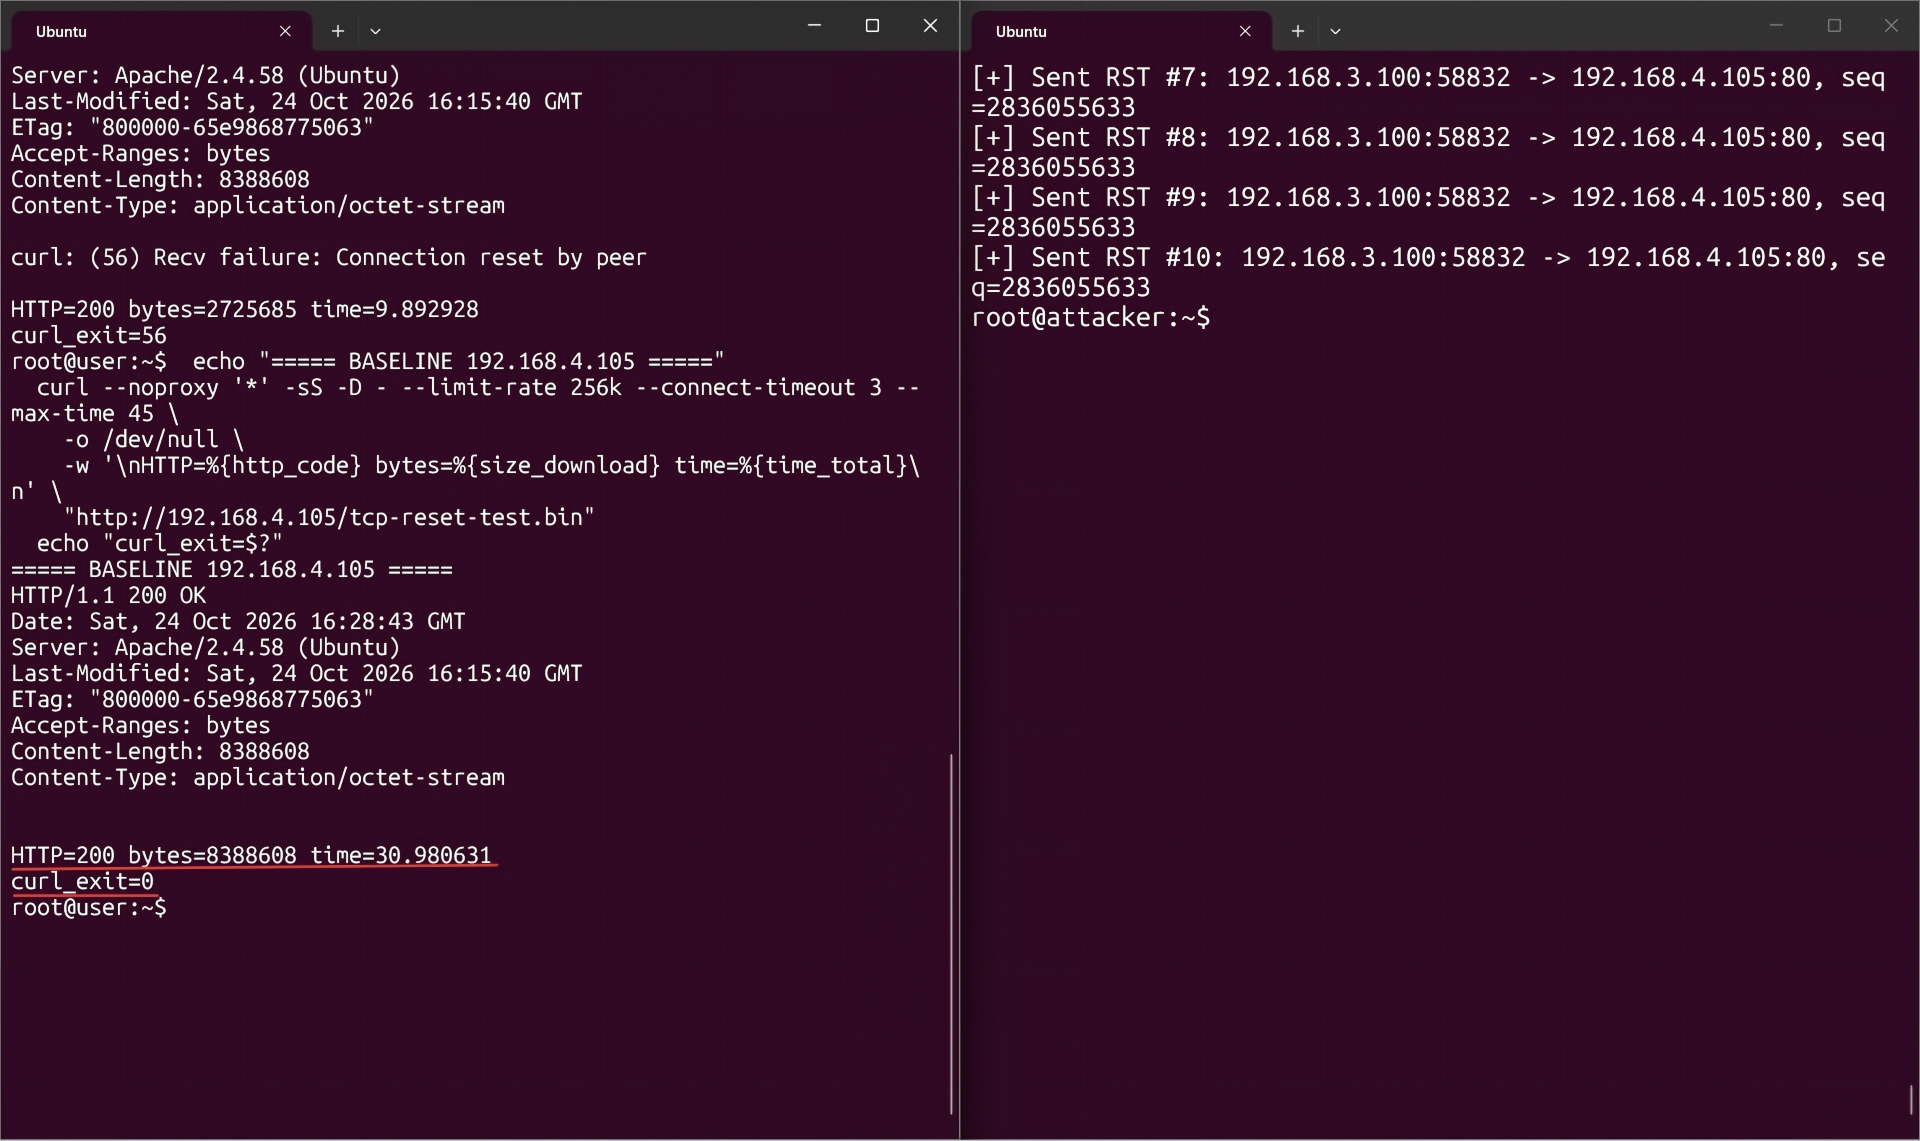
\includegraphics[trim=0 0 576bp 0,clip,width=0.76\linewidth]{figures/task3/http_recovery(1).png}
    \caption{停止 RST 监听后，受害者服务器的完整 \texttt{HTTP} 下载恢复}
    \label{fig:task3-recovery}
\end{figure}


\section{实验讨论}
\input{content/discussion.tex}

\section{参考资料}
% \nocite{labguide,rfc7616,scapy,wireshark}
% \printbibliography[heading=none]

\newpage
\appendix
\section{附录：关键代码}
\label{appendix:digest_crack}
% \input{content/append/key-code.tex}

\end{document}
